%%----------Chapter 2------------------------------------------
\chapter{Using Yeager to Generate Long Sequence Tests}
The test suite assembled in the previous chapter is an effective way for a software development team to verify that the core functionality of the system under test is fundamentally operational. When executed, it will test the few well-understood scenarios the testers wrote the suite for consistently and, assuming enough assertions are present, thoroughly. To accomodate new test scenarios will require an iteration of the entire process outlined in the previous chapter.

It is a boring, tedious, and repetitious task that can be the entire career of a test engineer. However, as any software engineer will know, tasks which are boring, tedious, and repetitious are ripe targets for computer automation, and the task of scenario authorship is no different.

This chapter will outline a method for adapting the existing test suite explored in the previous chapter, using a tool named Yeager, to enable the computer to generate scenarios automatically. Yeager is an MIT-licensed open source Python 3 module, with source available at \newline\url{https://github.com/elementc/yeager}. It provides a Python annotation and a set of utility functions. Usage of Yeager's state transition annotation allows testers to quickly and easily map an existing suite of test code onto a state machine, in the form of a graph. This graph can then be traversed using the utility functions, thereby generating new test scenarios from the existing code.

The resultant adapted test suite is published online at \url{https://github.com/elementc/monica-tests-yeagerized}.

\section{Software as a State Machine}
Consider the system under test, Monica. As a relationship management web site, it has a few obvious states it can be in: logged out and on the landing page, logged in and on the dashboard, viewing a list of contacts, viewing a list of journal entries, or viewing the settings page. This maps nicely to the page objects defined in the previous chapter. Actions on those page objects assume a current state (e.g., logged in and on the dashboard) and after execution are in a new state which may or may not be the same state. For instance, the \texttt{Dashboard.click\_contacts\_button()} method transitions from the dashboard to the contacts list, while the \texttt{AddPersonPage.set\_first\_name()} method should result in the system being in the same add-a-person page the system was on before the method was run.

Most modern programs can be looked at as systems composed of a finite set of states (pages, in this case) with some state transitions (links) and a data context (data entered into the system). Yeager uses this view to enable automated test sequence generation.

\subsection{States in The Example System}
Consider Monica's pages, which are already built into the test suite, to be states.

There are: the login page (\texttt{Login}) and logging in takes us to the \texttt{Dashboard} which has tabs for the \texttt{Contacts} list and the \texttt{Journal} log. There is also a \texttt{Settings} page which has subpages for \texttt{Import}, \texttt{Export}, \texttt{Users}, and \texttt{Tags}.

The Dashboard and Contacts list both let us \texttt{AddAContact}, while the Journal tab lets us \texttt{AddAJournalEntry}.

From a given \texttt{Contact}, there are pages where one can \texttt{AddASignificantOther}, \texttt{AddAChild}, \texttt{UpdateJobInformation}, \texttt{AddANote}, \texttt{AddAnActivity}, \texttt{AddAReminder}, \texttt{AddAGift}, and \texttt{AddADebt}.

For the purpose of these discussions, those pages will constitute the entire set of states in the system under test. Conveniently, each of them is represented as a Python class.

\begin{figure}
\noindent\makebox[\textwidth]{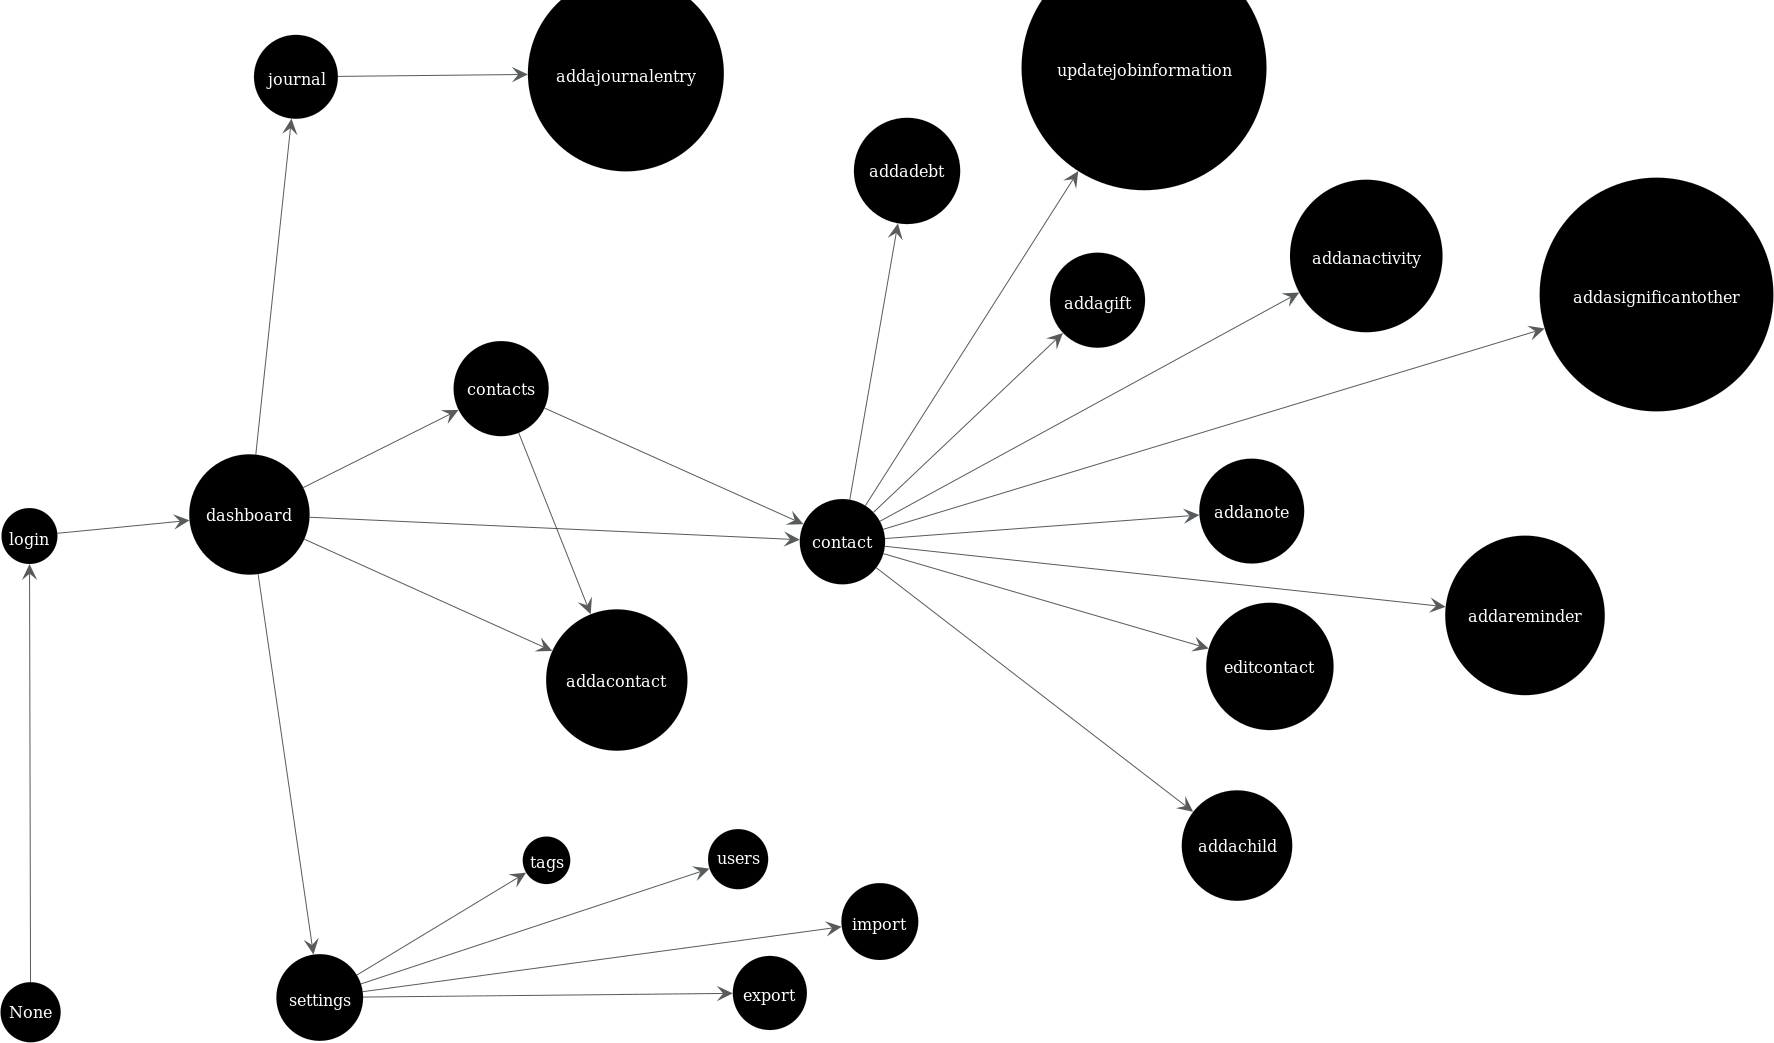
\includegraphics[width=\textwidth]{notionalstates}}
\caption{Notional States in the Monica System}
The states a tester might imagine to be in Monica, with lines connecting each state to the state that notionally lead to them, for instance the \texttt{Settings} page leading to the \texttt{Import} page. Note that connecting lines are merely explanatory, other connections exist between the actual states in the system, for instance in the form of a logout button on every page.
\end{figure}

\subsection{State Transitions as Actions in The Example System}
A graph consists of a set of nodes and a set of edges. If the nodes are the states the system under test may be in, the edges are the actions that may be taken from those states, possibly resulting in a state transition. It is certainly possible for an edge to be a loop connecting the starting state to itself. In the particular case of testing web applications, note that though it is reasonable to author a page object model with each method corresponding to an edge, this is not an assumption that is necessary to make, and would-be Yeager adopters may choose to lump lower-level page object methods into clusters of function calls in new functions and treat those higher-level functions as edges instead. The example Yeagerized Monica tests do just this, creating a suite of Yeager-friendly functions as snippets of existing test sequences, built from page object function calls.

\subsection{Capturing Contextual State}
Before embarking on the journey of high volume test automation that follows, it is important to consider the entirety of the software system. More than just software, a system includes the entire context of the software's execution, from the software itself, to the contents of the database, to the number of active system threads, to the ambient temperature of the room the system is running in.

Some of these are impossible to control for in a testing environment: it is unreasonable to unseat a CPU cooler to attempt to replicate a bug related to a developer's cousin's dust-clogged Pentium II, for instance. Others are possible to configure with initialization scripts and virtualization to a degree, for instance always having the same base OS image and environment variables, or always having the same amount of RAM and number of CPU cores. Still more can be controlled for using database snapshots and well-documented test data. Regardless, remembering these variables, which are external to the code but internal to the system under test, is critical to the development exercises in this chapter. \citep{HoffmanTradeoffs}

\subsection{Taking a Walk on the Graph}
Traditional test sequencing can be thought of as following a set of directions to traverse a map, akin to ``from A, go to B, turn right at C, stop at D'' and so on. These pre-planned scripts are an effective way to make sure the test visits all of the parts of the system that need testing at least once.

An additional exercise might be to go wandering: From a given state, pick a random transition that lists that state as the starting state, execute it, make a note of that transition's ending state as being the new current state, and repeat until some terminating conditions are met or the software under test crashes.

The notion of wandering around a program is a useful one for testing. First, it simulates human usage a little more realistically than many test scenarios: how many users actually start from a freshly booted computer, load up and login to the dashboard, create one record, search for that record, delete that record, then log out? Second, such a process can be of any arbitrary length which, while also contributing to a more realistic usage simulation\footnote{Consider that the author's instance of the Atom text editor has been open since August, while the typical Atom continuous integration instance takes 30 minutes to build the software and run all tests.\citep{CircleCI}}, permits test managers to use as much of the technique as they want to- wandering the program under test for a few hours on their laptop during a conference call or over a month on a virtual machine hosted in a private cloud somewhere.

\section{Yeager State Transition Annotations}
The meat of Yeager testing is accomplished through the annotation of Python test methods. An \textit{annotation}, also known as a \textit{decorator} or a \textit{function decorator} is a special Python function which is executed at the time of another function's definition, receives the function being defined as well as any other required items as parameters, and can optionally wrap the function being defined in a special modifier. Yeager is implemented as a special Python annotation and a set of utility functions which register after definition and can then call plain old Python functions.

The annotation, \texttt{yeager.state\_transition}, and some utility functions, \\\texttt{yeager.orphaned\_states} and \texttt{yeager.reachable\_states}, are described in this section.

A note on Python convention: there are two kinds of parameters a function may take. The first, \textit{positional arguments}, are passed like this: \texttt{print("some argument")} or \texttt{math.pow(3,2)}. The second, \textit{keyword arguments}, sometimes shortened to \textit{kwargs}, are passed like this:
\texttt{timedelta(hours=3, minutes=7)}. Order does not matter with kwargs. Positional arguments and kwargs that are not explicitly defined in a function's signature can both be captured for use by a function. Positional arguments are captured into a Python \texttt{list} by defining a (potentially semi-) final argument prefixed with a single asterisk, keyword arguments into a Python dictionary (\texttt{dict}) with a final argument prefixed with two asterisks, like this:
\\\texttt{def function(arg1="Default val", *args\_var, **kwargs\_var)}

\subsection{State Identifiers}
Anything that can be a Python \texttt{dict} key can serve as a state identifier. For simplicity's sake strings are used in this document, but as long as Python will allow it, so will Yeager. Enterprising Yeager hackers may use the actual Python page object model class, for instance.

The example implementation of a Yeager test uses unique strings for state identifiers. There is no strong reason for this, it is just illustrative.

\subsection{Basic State Transition Annotations}
The fastest way to get started with using Yeager is to define a function for each of the state transitions to be used in the test. These will probably be short snippets from the traditional-style test sequences. Then, for each of these functions, the \texttt{yeager.state\_transition} annotation should be to mark the transition of that function. Here is an example using some of the Monica test code from the previous chapter:

\begin{Verbatim}[fontsize=\small, baselinestretch=0.75]
from pages.login import LoginPage
from pages.dashboard import DashboardPage
from yeager import state_transition

@state_transition(None, "login-page")
def open(driver, **kwargs):
    driver = webdriver.Chrome()
    driver.get("https://app.monicahq.com/")

@state_transition("login-page", "dashboard-page")
def log_in(driver, **kwargs):
    login = LoginPage(driver)
    login.log_in_correctly()

@state_transition("dashboard-page", "login-page")
def log_out(driver, **kwargs):
    dashboard = DashboardPage(driver)
    dashboard.log_out()
\end{Verbatim}

Note that Python \texttt{None} constant is used as a reference to the uninitialized system. Yeager treats \texttt{None} as a special node in the implied state model the annotations provide: it is assumed to be the entry point, though that may be overridden.

\subsection{Verifying Connectedness}
Yeager provides a utility function to check for states which cannot be reached from a given state, probably due to misconfigured annotations. The function, \texttt{yeager.orphaned\_states}, takes one optional argument (the starting state, it defaults to \texttt{None}), and returns a \texttt{list} of all states that Yeager knows about but does not know how to get to. The inverse set, the known states, is also provided as a utility function with the same optional argument, as \\\texttt{yeager.reachable\_states}. Though the orphaned states function is useful for debugging, it can be used in other automated ways, for instance as a way to automate \texttt{walk} calls with each of the ``orphaned'' states being new entry points.

\section{Yeager Test Harnesses}
A suite of Yeager-annotated Python functions, while neat, is neither immediately useful (it is still just a chunk of naked functions), nor particularly intrusive (annotating a function with a Yeager state transition only adds a print statement before the function executes). Analysis of the state transition graph can be done manually for sure (\texttt{from yeager import nodes, edges}), but Yeager also provides a set of utility functions to actually exercise the system under test.

\subsection{Test Setup and Entry Point}
It is up to testers to generate Python scripts that start up and execute a Yeager test, but the process is straightforward.

The first step is to cause the Python interpreter to parse all of the relevant Yeager annotations. In simple test scripts, it is enough to simply write the test code and annotations at the top of the file, but in large test suites, it may be necessary to import those Python files at the top of the Yeager test script instead. Critically, Yeager annotation metadata exists as long as the Python interpreter instance does, so it does not matter what modules or other structure applies to the code the Yeager annotations are spread around in. If it has been parsed, Yeager knows about it.\footnote{Unless modifications have been made to the \texttt{nodes} or \texttt{edges} data structures.}

To actually start taking a walk on the state model, simply call Yeager's \texttt{walk} function.

\subsection{Walk Options and Execution}
The function \texttt{yeager.walk} takes some special arguments that determine how a test will eventually come to an end. If a tester just wants to go walking until they tell it to stop, they can call it with no args and it will run until the test is killed with a \texttt{SIGINT}. If a tester wants to just take a fixed number of steps, they can pass that as a naked integer or kwarg named count to \texttt{walk} and it will run for that many steps and then return. If a tester does not care about how long a test runs, and only wants to run until the program gets to some particular state, using the kwarg \texttt{exit\_state} with the desired end state will cause the \texttt{walk} call to return as soon as Yeager wanders to that state. And, finally, if a tester wishes to start the walking from a state other than the default starting state of \texttt{None}, they may do so by supplying the kwarg \texttt{start\_state} with the desired starting state.

All of these different preferences are just plans- the intended way to wander the graph. If an exception is raised in the underlying code, the exception is thrown all the way to the caller. Yeager does not try to continue walking since the system under test may be in a corrupt state. It is not possible to resume the existing \texttt{walk}, but it is possible to call \texttt{walk} again from scratch.

\subsection{Application Context}
All other kwargs that are passed to the \texttt{yeager.walk} call will be passed to the transition functions by Yeager, so a driver kwarg could be used to provide a webdriver to a web application's test suite, or a \texttt{dict} named context could store contextual information about the system under test.

Changes to mutable objects are preserved for the rest of execution, so it becomes possible to memoize things like data entered into the system or previously-captured search results. All kwargs unrecognized by the \texttt{walk} call are passed to all of the transition functions that Yeager steps through, so it is in the Yeager test style to have all test functions use the \texttt{**kwargs} catch-all argument in case a new context argument is added in the future of the test suite's development.

\subsection{Logging in Yeager}
Yeager does not make any particular assumptions about the logging toolkit that the tester may use. It uses standard output to print its own data, though future revisions might use the standard Python logging interface. For any high volume testing like in Yeager, it is very important to log with vigor, as a failure is often the result of many consecutive steps instead of one instant.

\subsection{Controlling the Path: Blacklists}
While it may seem counterintuitive after going to the effort to define them, it is possible to mark a state as one to not visit during a \texttt{walk}, or a transition as one not to take. This is useful, say, in cases where testers might want a run configuration that avoids certain known-buggy regions of the system under test, or try a Yeager test but know parts of their Yeager-specific code is still incomplete. It is accomplished by using the \texttt{yeager.add\_state\_to\_blacklist} and \texttt{yeager.add\_transition\_to\_blacklist} functions. Blacklisted states and transitions can be removed by using the \texttt{yeager.remove\_state\_from\_blacklist} and \texttt{yeager.remove\_transition\_from\_blacklist} functions.

\subsection{Controlling the Path: Weights}
Humans using software do not truly do actions equally randomly. A user of the Atom text editor, for instance, probably spends more time typing and saving than they do moving tabs around, opening consoles, running compile/lint commands, changing themes or settings, and so on. To enable better simulation of these more-probable actions, Yeager supports the notion of weighting edges.

An edge may be weighted by using a standalone function
\\(\texttt{yeager.set\_edge\_weight}) or by using the weight kwarg with the state transition annotation (\texttt{@state\_transition("st-a", "st-b", weight=10)}). Notionally, an unweighted edge has a weight of 1. This edge gets one entry into the pool of candidates for selection by the \texttt{walk} algorithm. An edge with a weight of 5 gets five entries into the pool. A final edge with a weight of 2 gets two entries into the pool. From the combined pool (with eight entries), one is chosen as a random draw and executed.

\section{Yeager in Action: Testing Monica}
With the Yeager package described in a general fashion, a detailed look is now taken at specific use case: testing the Monica personal CRM. Just as a reference traditional test suite was provided as the \texttt{monica-tests-traditional} repository, so too has a reference Yeager test suite been provided online at \url{https://github.com/elementc/monica-tests-yeagerized}.

\subsection{Detailed Test Code}

The following test code was used to generate the example runs which follow. It is a snippet of the reference Yeager suite, reformatted to run from a single file as opposed to the reference suite's full structure.

\begin{Verbatim}[fontsize=\small, baselinestretch=0.75]
from selenium import webdriver
from pages.login import LoginPage
from pages.dashboard import DashboardPage
from pages.header_page import HeaderPage
from pages.contacts import ContactsPage
from pages.add_a_contact import AddPersonPage
from pages.contact import ContactPage
from pages.edit_contact import EditContactPage
from yeager import walk
from yeager.annotations import state_transition
header_pages = ["dashboard-page", "contacts-page",
  "journal-page", "settings-page"]

@state_transition(None, "login-page")
def open(driver):
    driver.get("https://app.monicahq.com/")

@state_transition("login-page", "dashboard-page")
def log_in(driver):
    login = LoginPage(driver)
    login.log_in_correctly()

@state_transition(header_pages, "login-page")
def log_out(driver):
    header = HeaderPage(driver)
    header.log_out()

@state_transition(header_pages, "dashboard-page")
def dashboard_page(driver):
    header = HeaderPage(driver)
    header.go_dashboard()

@state_transition(header_pages, "contacts-page")
def contacts_page(driver):
    header = HeaderPage(driver)
    header.go_contacts()

@state_transition(header_pages, "journal-page")
def journal_page(driver):
    header = HeaderPage(driver)
    header.go_journal()

@state_transition(header_pages, "settings-page")
def settings_page(driver):
    header = HeaderPage(driver)
    header.go_settings()

@state_transition("contacts-page", "add-contact-page")
def add_someone(driver):
    contacts = ContactsPage(driver)
    contacts.click_add_person()

@state_transition("add-contact-page", "contacts-page")
def cancel_add(driver):
    add = AddPersonPage(driver)
    add.click_cancel_button()

@state_transition("add-contact-page", "contact-page")
def okay_add(driver):
    add = AddPersonPage(driver)
    add.click_add_button()

@state_transition("contact-page", "edit-contact-page")
def edit_contact(driver):
    contact = ContactPage(driver)
    contact.click_edit_contact()

walk(20, driver=webdriver.Chrome())

\end{Verbatim}

\subsection{Example of Execution: No Bugs}
Running the full code from the above section can yield a number of different outputs. Here is one run which terminates successfully.

\begin{Verbatim}[fontsize=\small, baselinestretch=0.75]
  executing <function open>, current state -> login-page
  executing <function log_in>, current state -> dashboard-page
  executing <function log_out>, current state -> login-page
  executing <function log_in>, current state -> dashboard-page
  executing <function dashboard_page>, current state -> dashboard-page
  executing <function dashboard_page>, current state -> dashboard-page
  executing <function log_out>, current state -> login-page
  executing <function log_in>, current state -> dashboard-page
  executing <function settings_page>, current state -> settings-page
  executing <function contacts_page>, current state -> contacts-page
  executing <function log_out>, current state -> login-page
  executing <function log_in>, current state -> dashboard-page
  executing <function journal_page>, current state -> journal-page
  executing <function log_out>, current state -> login-page
  executing <function log_in>, current state -> dashboard-page
  executing <function log_out>, current state -> login-page
  executing <function log_in>, current state -> dashboard-page
  executing <function contacts_page>, current state -> contacts-page
  executing <function add_someone>, current state -> add-contact-page
  executing <function cancel_add>, current state -> contacts-page
\end{Verbatim}

No error message appears, and the test exits after 20 steps, the requested exit condition. This is a successful, if short, test.

\begin{figure}[h]
\noindent\makebox[\textwidth]{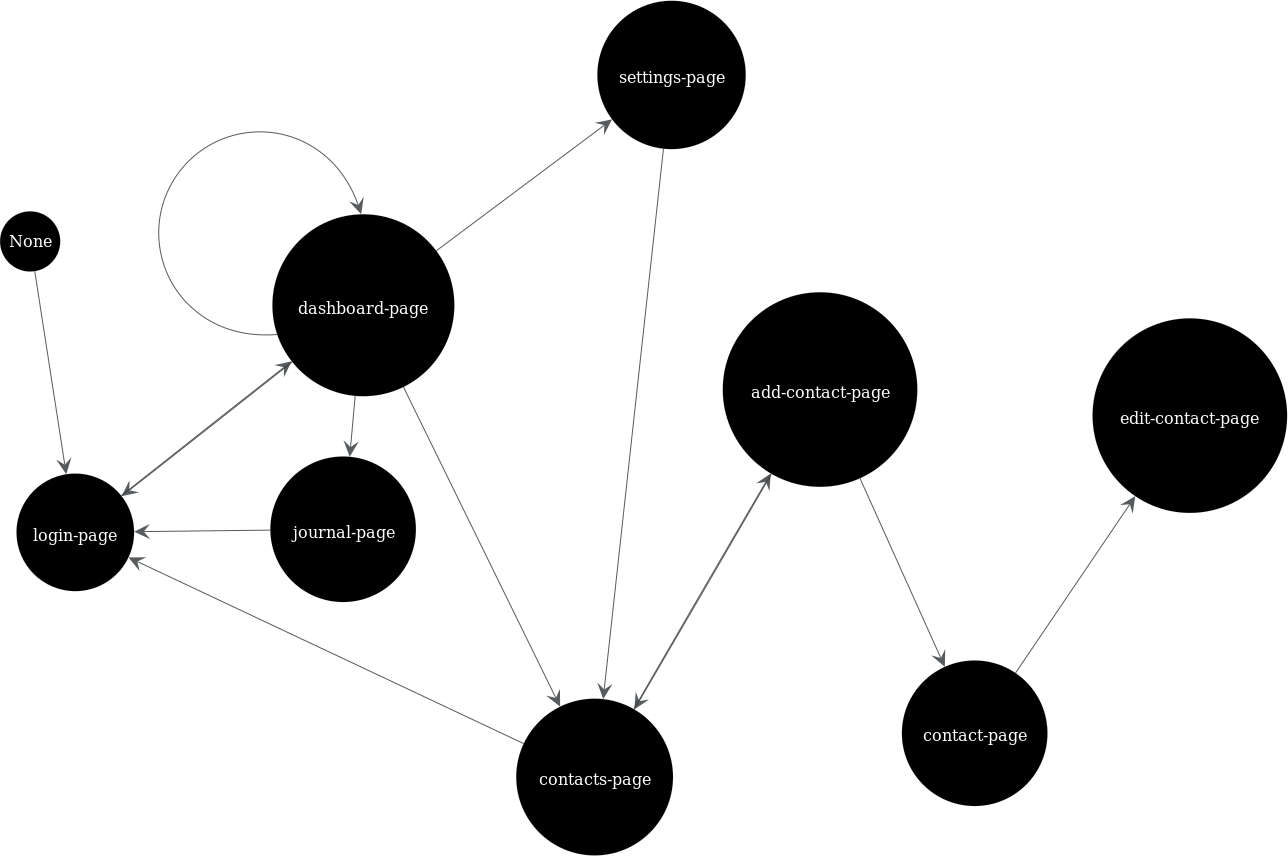
\includegraphics[width=\textwidth]{traceme}}
\caption{States and Transitions in the Example Test Runs}
This graph is a subgraph of the total inferred system state model, representing every node and edge used in the test runs in sections 2.4.2 and 2.4.3. Edges are unlabelled but correspond to functions named in the corresponding sections.
% for der fingerpoken
\end{figure}


\subsection{Example of Execution: Bug In Model}
Sometimes, a test fails. Yeager makes no guarantee that a test failure is consistent with a fault in the software. In fact, the only thing it guarantees is that the model does not match the software's behavior. This could just as likely represent a fault in the model that Yeager inferred. Here is one such example:

\begin{Verbatim}[fontsize=\small, baselinestretch=0.75]
executing <function open>, current state -> login-page
executing <function log_in>, current state -> dashboard-page
executing <function contacts_page, current state -> contacts-page
executing <function add_someone>, current state -> add-contact-page
executing <function okay_add>, current state -> contact-page
executing <function edit_contact>, current state -> edit-contact-page
(traceback omitted)
selenium.common.exceptions.NoSuchElementException:
  Message: no such element:
    Unable to locate element:
    {"method":"link text","selector":"Edit contact information"}
    (Session info: chrome=63.0.3239.59)
    (Driver info: chromedriver=2.32.498550,
    platform=Windows NT 10.0.15063 x86_64)
\end{Verbatim}

The test begins well enough, then dives into creating a contact. It opens the add-a-contact page, and then directly tries to add the (empty) contact. The next step it takes, trying to open the just-added contact for editing, throws a NoSuchElement exception! That is because the  ``add this contact'' button did not actually transition the system to the contact-page state, instead showing an error message. This is a common failure mode in Yeager tests, it does not represent a bug in the software so much as a bug in the test code: there is an implicit requirement that the add-contact-page state must have a string put into the first name field before the add button will work as expected. This can be mitigated by using a separate pseudo-state (``add-contact-page'' and ``add-contact-page-filled'') or through runtime manipulation of the Yeager blacklist, namely by blacklisting the \texttt{okay\_add} transition at the end of the \texttt{add\_someone} function and then removing it from the blacklist once the first name field gets something put into it.

\subsection{What a Bug In Software Looks Like}
Actual bugs in the software under test will appear nearly identically to the case of bugs in the Yeager model.

When a bug crops up, it will present as a sequence of calls that result in a failed assertion. As in the model bug above, the actual fault happened before the step that the assertion took place in, and it is simply the case that the next step couldnt run because it was in an unexpected state.

Testers will know a bug in the software if the steps leading up to that failure are sensible, that is, if there is no logical error in the steps that led to the state transition that failed. Defensive testers will write an exception handler around their walk call that dumps the state of the system under test at the moment of the inspection, so as to ease verification of suspected failures.

\subsection{Visualizing an Inferred State Graph}

As Yeager stores a computer representation of the system's state graph to operate, it is simple to export this graph for visualization from other tools. The following code will render a graph using the popular \texttt{graph\_tool} package.

\begin{Verbatim}[fontsize=\small, baselinestretch=0.75]
  rom yeager import nodes, edges
  from graph_tool.all import *

  # import yeager transitions here.

  def graph():
      g = Graph()
      g.set_directed(True)

      y_node_map = {}
      v_node_map = g.new_vertex_property("string")
      e_map = g.new_edge_property("string")

      for node in nodes:
          v = g.add_vertex()
          y_node_map[node] = v
          v_node_map[v] = str(node)

      for src in edges.keys():
          for dest in edges[src]:
              e = g.add_edge(y_node_map[src], y_node_map[dest[0]])
              e_map[e] = str(dest[1])

      # pos = radial_tree_layout(g, y_node_map[None])
      # pos = sfdp_layout(g)
      # pos = random_layout(g)
      # pos = fruchterman_reingold_layout(g)
      pos = arf_layout(g)
      graph_draw(g, pos=pos, vertex_text=v_node_map, edge_text=e_map)
\end{Verbatim}

The commented-out ``\texttt{pos =}'' lines are ways to call different layout algorithms provided by the package. Different types of software will benefit from different layouts, and manual layout can be achieved through the \texttt{graph\_tool}'s interactive window function. Multiple edges that connect the same start and end nodes will be drawn on top of each other under the default settings, and consequently their labels may also overlap. This can be mitigated through modification of the rendering settings in the call to \texttt{graph\_draw}.

The graphics used in the previous sections were generated through modifications of this example code, as was the following graphic capturing a subset of the state model inferred from the \texttt{monica-tests-yeagerized} repository.

\begin{figure}
  \noindent\makebox[\textwidth]{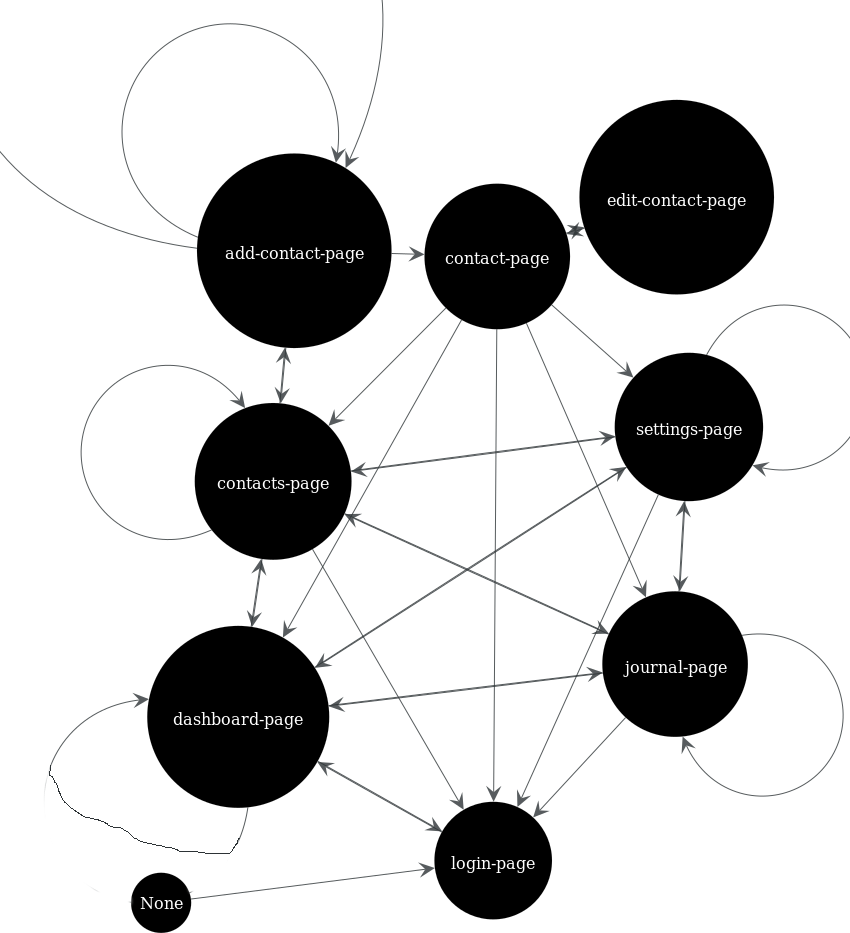
\includegraphics[width=\textwidth]{monicamodel}}
  \caption{Subgraph from \texttt{monica-tests-yeagerized}}
  Edge labels have been turned off for legibiity, and aspect ratio has been modified.
\end{figure}
